\section{The Neighbor Joining Algorithm}

Neighbor joining is a particular method of hierarchical clustering for phylogentic tree construction. In this problem, we are given a bunch of species with ``distances'' between them, where $d(i,j)$ is the distance between species $i$ and $j$, that represent how different they are from each other. It is specifically an agglomerative method, meaning that it starts with individual clusters for each species, and then iteratively merges the clusters into superclusters, eventually converging on a single cluster. We can depict this graphically as a binary tree, where each leaf is a species, and all the internal nodes represent the joining of two clustesr. This can be seen in Figure \ref{tree}, and is more generally called a {\em dendrogram}.

\begin{figure}[h!]\label{tree}
  \caption{A phylogenetic tree is an example of a dendrogram.}
  \begin{center}
    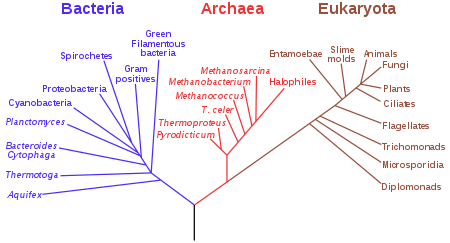
\includegraphics[width=8cm]{phylogenetictree.png}
  \end{center}
\end{figure}

In neighbor joining, we start at the bottom of this tree and construct one internal node at a time working up the tree. Ideally, we want species that are more similar to be grouped closer in the tree, as in, they diverged more recently in evolutionary history. We do this by creating a sort of proxy for distance and store it in what we call a $Q$ matrix. This matrix represnts the taxa we are currently looking to merge, so if we have $t$ taxa, it will be a $t\times t$ matrix. The $i,j$th entry of $Q$ corresponds to this distance proxy between taxa $i$ and $j$. The proxy is as follows.

\begin{align}\label{qformula}
Q(i,j) = (n-2)d(i,j) -\sum_{k=1}^n d(i,k) - \sum_{k=1}^n d(j,k).
\end{align}


Intuitively, this is simply the distance between the two species minus all the distances between each of the two species and all others, where the distance between the two species is weighted much larger. Therefore, $Q(i,j)$ is small if $d(i,j)$ is small relative to the average distances between $i$ and all other species, as well as $j$ and all other species. We want this distance to be small, meaning these species are similar relative to other species.

In the actual algorithm, we start by calculating our $Q$ matrix across all species. We then find the minimum value in $Q$, say $Q(i,j)$, and then merge species $i$ and $j$. Now we will ignore species $i$ and $j$ because we have found the vertex directly above them in the dendrogram. They are replaced by a single new taxa that represents the cluster of $i$ and $j$ together.

To calculate the distance between $u$ and both of its children $i$ and $j$, we use the following method.

\[d(u,i) = \frac12d(i,j) + \frac1{2(n-2)} \left[\sum_{k=1}^n d(i,k) + \sum_{k=1}^n d(k,j)\right].\]

We now need to find the distance between the new taxa and all the other taxa currently in question. Say $i$ and $j$ are the taxa we merged, and $u$ is the new one, and we want to calculate the distance between $u$ and some $k$. Because our graph is additive, we want the sum of the paths from $i$ to $k$ and $j$ to $k$ to be consistent on the graph we are constructing. The first path has length $d(i,k) = d(i,u) + d(u,k)$, and the second has length $d(j,k) = d(j,u) + d(u,k)$. Combining these together, we get the following.

\begin{align}\label{distances}
d(u,k) = \frac12[d(i,k) + d(j,k) - d(i,j)].
\end{align}

Now we have all the new distances for the next iteration in the tree and are ready for the next iteration. We continue through this process, keeping track of the vertices we merge until we have constructed our entire tree.

An interesting property of the tree we construct comes from this notion of keeping the graph additive. In our resulting tree, note that we have each branch distance as represented by the $d$ of adjacent vertices in the corresponding steps of the algorithm. It then holds true, by construction of the tree, that $d(i,j)$ for any species $i$ and $j$ is equal to the path length in the resulting tree. Because of this, if we initially derive our distances based off of some input tree $T$, then neighbor joining will output a tree that agrees with it.

This algorithm is polynomial time, but it is unclear if the runtime can be improved while keeping the same structure. It requires $\mathcal{O}(n)$ iterations, and each iteration requries $\mathcal{O}(n^2)$ computations to compute $Q$ and recompute distances. Therefore, it runs in $\mathcal{O}(n^3)$ time. We are interested in improving this.


